\documentclass[12pt, spanish, oneside, onecolumn, a4paper]{report}
\usepackage[spanish,activeacute]{babel}
\usepackage[latin1,utf8]{inputenc}
\usepackage{times}
\usepackage[T1]{fontenc}
\usefont{T1}{arial}{m}{n}
\oddsidemargin 0in
\textwidth 6.75in
\topmargin 0in
\textheight 8.5in
% \parindent 0em
\parskip 2ex

\usepackage{fancyheadings}
\headheight 35pt
\usepackage{graphicx}
\usepackage[colorlinks=true, urlcolor=blue, filecolor=green,
linkcolor=red, pdfkeywords={}, pagebackref, pdfpagemode=UseOutlines,
bookmarksopen=true]{hyperref}

\usepackage{tabularx}
\usepackage{colortbl}
\usepackage{wrapfig}

\usepackage{tabulary}
\setlength\tymin{699pt}
\setlength\tymax{700pt}
\setlength\doublerulesep{0.5px}

\graphicspath{{./img/}}

\usepackage{epic}
\makeatletter

\renewcommand{\contentsname}{Indice}
\renewcommand{\appendixname}{Apéndice}
\renewcommand{\figurename}{Figura}
\renewcommand{\listfigurename}{Indice de figuras}
\renewcommand{\tablename}{Tabla}
\renewcommand{\listtablename}{Indice de tablas}

% un comando
\def\comando#1{

\begin{tabulary}{620px}{|>{\columncolor[rgb]{0.8,0.9,0.8}}L|}
  \hline \textsl{#1}\ \hline
\end{tabulary}

}

% varios comandos
\newenvironment{command} {

  \tabulary{420px}{*{2}{|>{\columncolor[rgb]{0.8,0.9,0.8}}L}|}
  % \hline
  \textbf{portage:} & \textbf{entropy:}\tabularnewline } {
  % \hline
  \endtabulary

}
% end comandos

\usepackage[toc,nonumberlist]{glossaries}
\makeglossaries

%\begin{titlepage}
%\newcommand{\HRule}{\rule{\linewidth}{0.5mm}} % Defines a new command for the horizontal lines, change thickness here
%\center % Center everything on the page
%
%%\textsc{\LARGE University Name}\\[1.5cm] % Name of your university/college
%%\textsc{\Large Major Heading}\\[0.5cm] % Major heading such as course name
%%\textsc{\large Minor Heading}\\[0.5cm] % Minor heading such as course title
%\HRule \\[0.4cm]
%{ \huge \bfseries Git}\\[0.4cm] % Title of your document
%\HRule \\[1.5cm]
%\begin{minipage}{0.4\textwidth}
%\begin{flushleft} \large
%\emph{Author:}\\
%Ing. Anielkis \textsc{Herrera} % Your name
%\end{flushleft}
%\end{minipage}
%~
%\begin{minipage}{0.4\textwidth}
%\begin{flushright} \large
%%\emph{Supervisor:} \\
%%Dr. James \textsc{Smith} % Supervisor's Name
%\end{flushright}
%\end{minipage}\\[4cm]
%{\large \today}\\[3cm] % Date, change the \today to a set date if you want to be precise
%%\includegraphics{Logo}\\[1cm] % Include a department/university logo - this will require the graphicx package
%\vfill % Fill the rest of the page with whitespace
%\end{titlepage}

\makeatletter
\def\maketitle{%
  \null
  \thispagestyle{empty}%
  \vfill
  \begin{center}\leavevmode
    \normalfont
    
\includegraphics{logo.png}\\[1cm]
%    {\LARGE \@title\par}%
    \vskip 1cm
    {\Large \@author\par}%
    \vskip 1cm
    {\Large \@date\par}%
  \end{center}%
  \vfill
  \null
  \cleardoublepage
  }
\makeatother


\begin{document}
\pagestyle{fancy}
\lhead{
\includegraphics[width=3cm,keepaspectratio=true]{logo.png}
%\includegraphics[width=3cm,keepaspectratio=true]{emblema-2008.eps}
}
%\cfoot{ \itshape{Carretera a San Antonio de los Baños. Km 5 {1/2}
% Reparto Torrens. Boyeros. Ciudad Habana.  Teléfono (53 7) 8372519
% e-mail: decano.f10@uci.cu }\newline \thepage}

\title{ Git }
\date{ \today\ }
\author{ Ing. Anielkis Herrera }

\pagenumbering{roman}
\maketitle

%\begin{abstract}
%Guía de uso de la herramienta Git para control de versiones
%\end{abstract}

\newpage
\pagenumbering{arabic}


\chapter{Introducción a Git}
\label{chap:intro}


\newacronym[longplural=Sistemas de Control de Versiones]{scv}{SCV}{Sistema de Control de Versiones}
\newacronym[longplural=Sistemas de Control de Versiones Distribuido]{scvd}{SCVD}{Sistema de Control de Versiones Distribuido}

%\newglossaryentry{scv}
%{
%  description={Sistema de Control de Versiones, sistemas utilizados para gestionar versionado en el desarrollo de software o documentación}
%}

%\newglossaryentry{Linux}
%{
%  description={es un término genérico que se refiere a la familia de sistemas operativos ``parecidos a Unix'' que utilizan el núcleo Linux}
%}

Git es un \gls{scvd}, desarrollado como sistema de software libre y diseñado para manejar desde proyectos pequeños hasta muy grandes, con gran rapidez y eficiencia.

Git es fácil de aprender y tiene una huella pequeña en el sistema, con un rendimiento increíblemente rápido. Supera a otros \glspl{scv} como Subversion , CVS , Perforce y ClearCase con características como trabajo con ramas locales, áreas de ``puesta en escena'' muy convenientes, y varios estilos de flujo de trabajo.


\section{Acerca de Git}
\label{sec:aboutgit}

\subsection{Creación y fusión de ramas}
\label{sec:branchingandmerging}

La función de Git que realmente lo hace destacar de entre la mayoría de los \gls{scv} es su modelo de ramificación. Git permite y alienta a tener varias ramas locales que pueden ser completamente independientes una de otra. La creación, fusión y supresión de las líneas de desarrollo toma solo unos instantes de segundo.

Esto significa que se pueden hacer cosas como:
\begin{description}
\item [Cambio de contexto sin fricción:] crear una rama para probar una idea,
adicionar contenido al historial un par de veces, volver a la rama desde donde se ramificó, aplicar un
parche, cambiar de nuevo a donde se está experimentando, y fusionar las ramas para adicionar los cambios del experimento a la rama original.
\item [Líneas de desarrollo separadas en roles:] tener una rama que siempre contiene sólo lo que va a la producción, otra a dónde se fusionan el código en que se ha trabajado, para probarlo, y varios más pequeños para el día a día.
\item [Función de flujo de base:] crear nuevas ramas para cada nueva característica en que se esté trabajando por lo que perfectamente puede alternar entre ellas, y a continuación eliminar cada rama cuando esta característica se fusione en la línea principal.
\item [Experimentación desechable:] crear una rama en la que experimentar , darse cuenta de que no va funcionar el experimento, y simplemente eliminarla - el abandono de un trabajo fallido que nadie más va a ver.
\end{description}

\begin{figure}[hb]
  \caption{Ramas en Git.}
  \centering
  
\includegraphics[width=.7\textwidth,keepaspectratio=true]{branches.png}
\end{figure}

En particular, cuando se ``empuja'' (\emph{\textbf{push}}) a un repositorio remoto, no es necesario hacerlo a todas las ramas. Se puede elegir compartir sólo una de las ramas, unas pocas de ellas o todas ellas. Esto permite probar nuevas ideas sin preocuparse de tener que planificar cómo y cuándo se va a fusionar o compartirlas con otros. Como se podrá ver posteriormente, se puede compartir la rama con otro desarrollador, con el que se puede trabajar en esa idea, sin necesidad de adicionarla al repositorio central.

Hay maneras de lograr algo de esto con otros sistemas, pero la obra en cuestión es mucho más difícil y propensa a errores. Git hace este proceso muy fácil y esto cambia la forma en la mayoría de los desarrolladores trabajan cuando lo aprenden.


\subsection{Pequeño y rápido}
\label{sec:smallandfast}

Git es rápido. Con Git, practicamente todas las operaciones son realizadas localmente, dandole una gran ventaja sobre los \gls{scv} centralizados que constantemente tienen que comunicarse con el servidor.

Git fue hecho para trabajar con el núcleo Linux, lo que sifnifica que tiene que trabajar eficientemente con repositorios de código muy grandes desde el primer día. Git está escrito en \textbf{C}, reduciendo la carga de ejecución asociada a lenguajes de alto nivel. La velocidad y el rendimiento son algunos de los principios seguidos desde los inicios de su diseño.

\subsection{Distribuido}
\label{sec:distributed}

Una de las mejores características de cualquier \gls{scvd}, Git incluído, es que es precisamente ``distribuido''. Esto significa que en lugar de hacer un ``checkout'' de la punta actual del código fuente, se hace un ``clon'' de todo el repositorio.

\subsubsection{Múltiples copias de seguridad}
\label{sec:multiplebackups}

Esto significa que aún si se utiliza un flujo de trabajo centralizado, cada usuario es esencialmente una copia de seguridad del servidor principal. Cada una de estas copias puede ser utilizada para sustituir el servidor central en caso de fallo o corrupción. En efecto, no hay un solo punto de fallo utilizando Git, a no ser que sólo se use una copia del repositorio.

\clearpage
\subsubsection{Cualquier flujo de trabajo}
\label{sec:anyworkflow}

Debido a la naturaleza distribuida de Git y un magnífico sistema de ramificación, un número casi infinito de flujos de trabajo se puede implementar con relativa facilidad.



\paragraph{Flujo de trabajo estilo Subversion:}


\begin{wrapfigure}{r}{0.65\textwidth}
  \begin{center}
    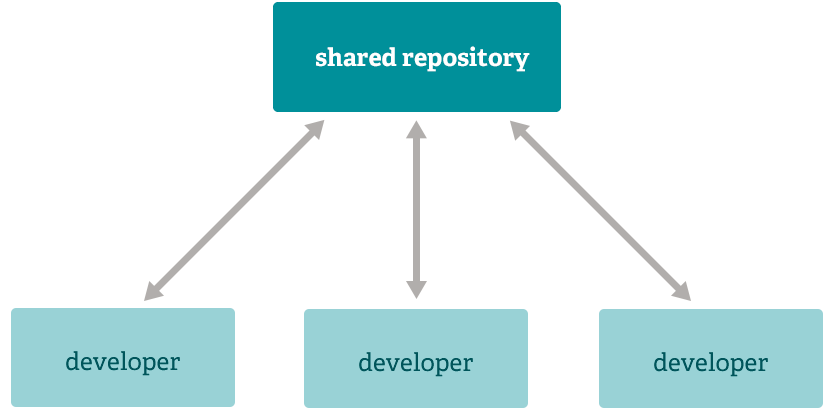
\includegraphics[width=.6\textwidth,keepaspectratio=true]{workflow-a.png}
  \end{center}
  \caption{Modelo centralizado estilo Subversion.}
\end{wrapfigure}
Un flujo de trabajo centralizado es bastante común, especialmente para personas cambiando desde sistemas centralizados. Git no permite que se ``empuje''(hacer \textbf{\emph{push}}) al servidor si alguien lo ha hecho desde la última vez que se descargó de él, por lo que un modelo centralizado donde todos los desarrolladores hacen \textbf{\emph{push}} al mismo servidor funciona bien.

% \begin{figure}[hb]
%   \caption{Modelo centralizado estilo Subversion.}
%   \centering
%   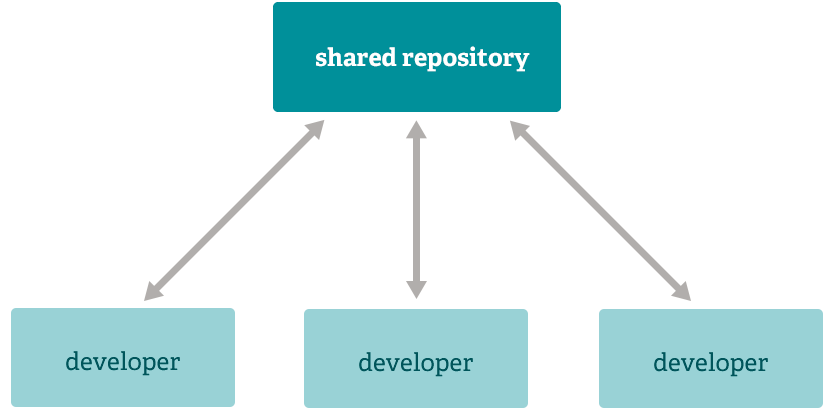
\includegraphics[width=.6\textwidth,keepaspectratio=true]{workflow-a.png}
% \end{figure}

\paragraph{Flujo con gerente integrador:}


\begin{wrapfigure}{r}{0.65\textwidth}
  \begin{center}
  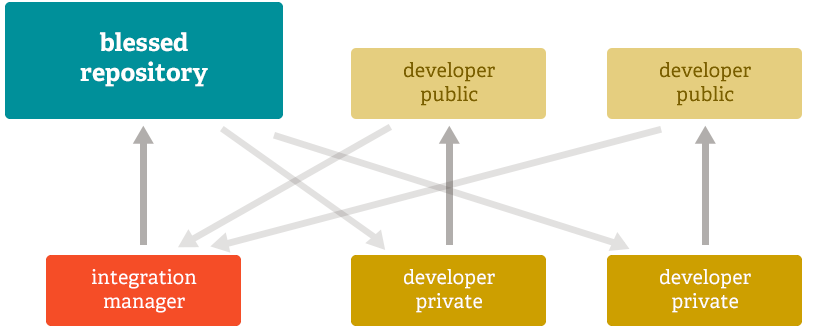
\includegraphics[width=.6\textwidth,keepaspectratio=true]{workflow-b.png}
  \end{center}
  \caption{Modelo con gerente integrador.}
\end{wrapfigure}
Otro flujo de trabajo, común en Git, consiste en un gestor de integración - una sola persona que es quien puede adicionar al repositorio ``bendecido''(el \emph{repositorio principal del sistema}). Un número de desarrolladores luego de clonar ese repositorio, empujan a sus propios repositorios independientes , y piden al integrador que revise y fusione sus cambios a ese repositorio. Este es el tipo de modelo de desarrollo visto a menudo con software libre o repositorios en \textbf{Github}.


%\begin{figure}[hb]
%  \caption{Modelo centralizado estilo Subversion.}
%  \centering
%\end{figure}

\paragraph{Flujo basado en un dictador y sus lugartenientes:}



\begin{wrapfigure}{r}{0.65\textwidth}
  \begin{center}
  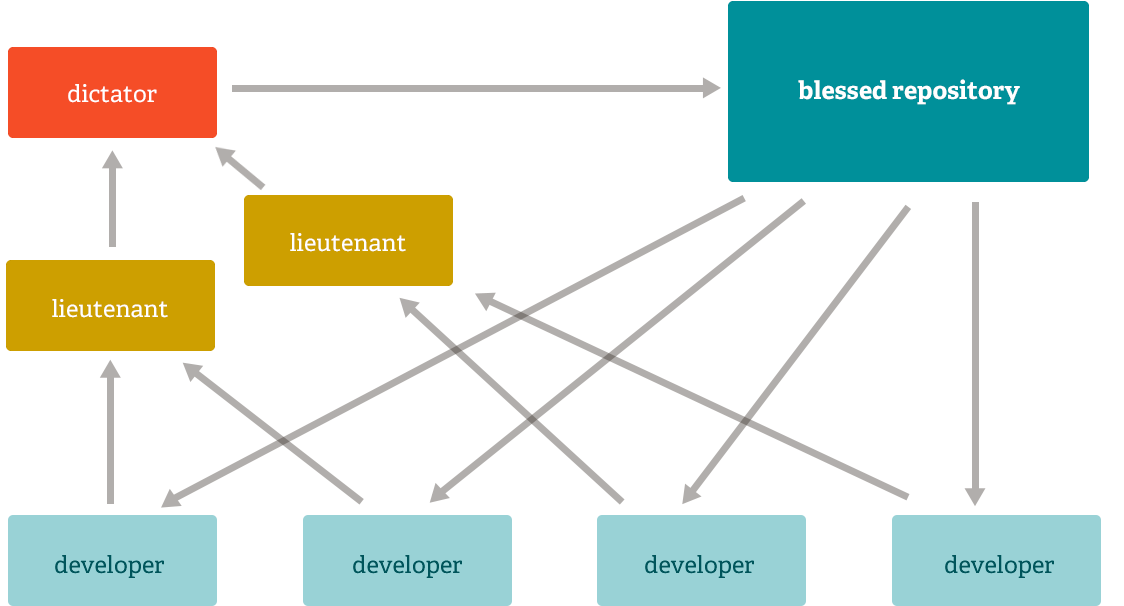
\includegraphics[width=.6\textwidth,keepaspectratio=true]{workflow-c.png}
  \end{center}
  \caption{Modelo con dictador y lugartenientes.}
\end{wrapfigure}
Para proyectos más grandes, un flujo de trabajo de desarrollo como el del núcleo Linux es a menudo eficaz. En este modelo, algunas
personas ( ``lugartenientes'' ) están a cargo de un subsistema específico del proyecto y fusionan todos los cambios relacionados con ese subsistema. Otra integrador (el ``dictador'' ) puede extraer los cambios sólo de sus lugartenientes (luego que estos los revisaron e integraron a sus subsistemas) y luego empujar al repositorio ``bendecido'' de dónde todo el mundo usa para trabajar.


% \begin{figure}[hb]
%   \caption{Modelo centralizado estilo Subversion.}
%   \centering
%   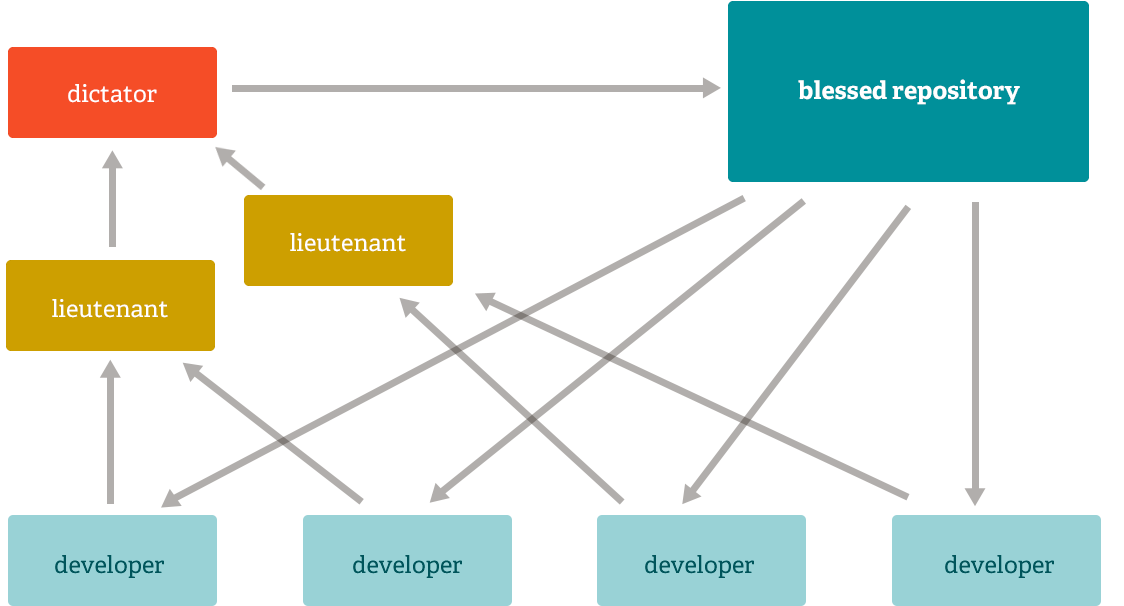
\includegraphics[width=.6\textwidth,keepaspectratio=true]{workflow-c.png}
% \end{figure}


\glsaddall
\printglossaries

\end{document}
